% main.tex, to be used with thesis.tex
% This contains the main work of your thesis.

%\bibliography{thesis}  % uses the references stored in Chapter1Radar.bib

\chapter{Data Persistence for Sensor Networks: A Case Study for NetBEAMS}
\label{chap:netbeams-overview}

As discussed in chapter 2, different properties of a sensor network and the
nature of the collected data must be taken into account in order to provide a
data persistence layer for a given sensor netwokr. Similarly, in order to
better assist one analysis of such functionality, chapter 3 proposed a set of
data persistence taxonomies related to different properties of the collected
data life cycle. In this way, the goal of this chapter is to describe the
fundamental properties of the case study used for this work, that is, NetBEAMS,
in order to ``set the stage'' for the selection of a database technology for it.
In this way, given the fact that NetBEAMS provides an automated infrastructure
solution for SF-BEAMS, this last component will be covered first. Then, this
work proposes a categorization of NetBEAMS to the face of the taxonomies, and
finally discusses the discusses the requirements for a data persistence.

\section{SF-BEAMS: a Marine Sensor Network for Water Quality Monitoring}

As described by \cite{netbeams2009}, NetBEAMS is a joint venture between the
department of Biology and Computer Science at San Francisco State University,
whose goal was to automate the operational execution of SF-BEAMS. On the other
hand, the San Francisco Bay Environmental Assessment and Monitoring Station, or
SFBEAMS \cite{sfbeams2006}, is an instance of an environmental sensor
network whose primary focus is the study of complex marine and estuarine
environments using the SF-BEAMS sensors. The network is deployed offshore of
its pier located on the banks of the San Francisco Bay at the Tiburon Island,
California, being operated by the department of Biology from San Francisco
State University. In this way, NetBEAMS is an experimental component that
utilizes the SF-BEAMS infrastructure to operate. This section details SF-BEAMS
in general, and presents the requirements for data persistence.

\subsection{The SF-BEAMS Infrastructure}

The SF-BEAMS sensor network is responsible for providing data for water quality
monitoring, as well as weather and surface conditions. Figure
\ref{fig:sf-beams} shows a picture taken from the SF-BEAMS web-camera.

\begin{figure}[!t]
  \centering
    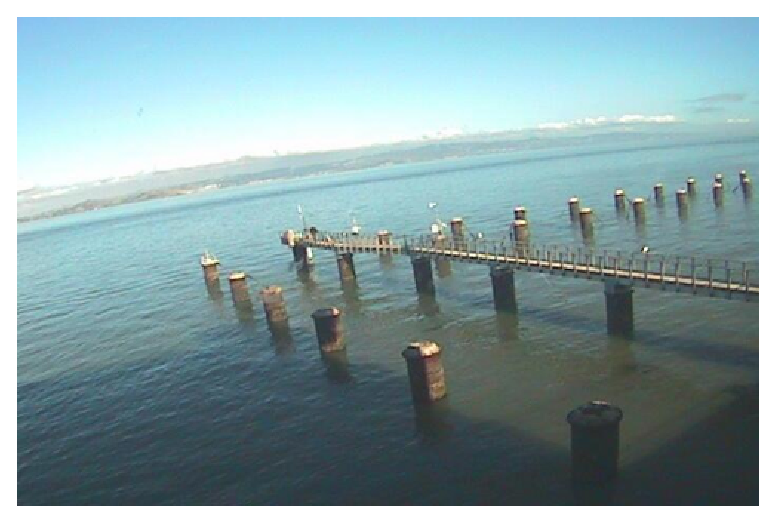
\includegraphics[scale=0.7]{../diagrams/cam_image-oct15}
  \caption{Picture of the SF-BEAMS Network, at the RTC pier. Tiburon, CA.}
  \label{fig:sf-beams}
\end{figure}

In general, the SF-BEAMS network infrastructure contains varying a number of
wired and wireless devices standing on pylons docked at the pier. Each of them
is responsible for observing different conditions of the area, having its own
mechanisms for internal storage for the collected data. In this way, data can
be directly transferred to the labs via Ethernet cables or collected manually
with a laptop computer.

\subsection{SF-BEAMS produced data and collection process}
\label{sec:sfbeams}

As described in section \ref{sec:sn-infrastructure}, sensor devices produce
its observed data based on properties of measurements defined by its
manufacturer. One example of such sensors is the ``YSI 6600 ESD V2", as seen in
Figure \ref{fig:ysi-device}. It is a powerful water quality monitoring device,
capable of producing around 52 bytes on a single real-time data stream reading,
as shown on Table \ref{tab:ysi-data-stream}.

\begin{figure}[!b]
  \centering
  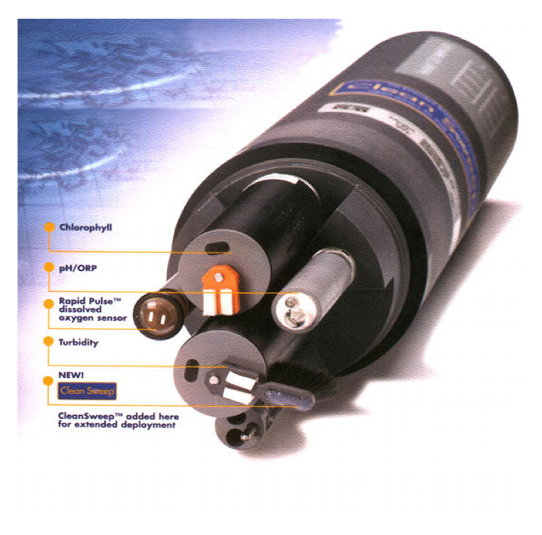
\includegraphics[scale=0.7]{../diagrams/ysi-device}
  \caption{Picture of the case study sonde device: YSI 6600 ESD V2}
  \label{fig:ysi-device}
\end{figure}

\begin{table}[!b]
    \caption{YSI Data Stream}
    \begin{center}
        \begin{tabular}{lr}
  12.20    192    179 5588.40   0.09   0.084   0.059  7.98   -79.6   99.5  8.83 
  0.4     8.7
        \end{tabular}
    \end{center}
    \label{tab:ysi-data-stream}
\end{table}

In order to have access to the observed data, the network staff downloads the
data using one of the device's connection such as the RS-232 serial connector
\cite{rs232}. Then, the RTC labs receives the collected data transferred from
the sensor devices to be used for archival purposes. According to one of its
staff members, the infrastructure of the SF-BEAMS in was comprised of
the following components (as of May 2009):

\begin{itemize}
  \item 5 YSI Sonde devices, among others, in operation at the RTC pier;
  \item The sampling frequency rate is configured in ranges of either 1, 6 or
  15 minutes, depending on the specification;
  \item The processed data, used for distribution over the Internet, is
   contains information regarding the time of the data collection.
\end{itemize}

Considering the infrastructure aforementioned, the data load in the server-side
of the RTC's laboratories produced by the YSI sonde sensors devices can be
estimated by analyzing the data distribution over a period of one year, as
shown in Table \ref{tab:ysi-data-distribution}:

\begin{table}[!b]
    \label{tab:ysi-data-distribution}
    \caption{Amount of data produced by the RTC's YSI sondes}
        \begin{center}
        \begin{tabular}{|c|c|c|c|c|c|c|}\hline 
        \textbf{YSIs} & \textbf{Rate} & \textbf{Hourly} & \textbf{Daily} &
        \textbf{Weeky} & \textbf{Monthly} & \textbf{Yearly}\\\hline 
        1 & 1 min & 3.04 Kb & 73.12 Kb & 511.87 Kb & 1.99 Mb & 23.99 Mb\\\hline 
        5 & 6 min & 15.23 Kb & 365.62 Kb & 2.5 Mb & 9.99 Mb & 119.97 Mb\\\hline 
        1 & 15 min & 0.5 Kb & 12.18 Kb & 85.31 Kb & 341.25 Kb & 3.99 Mb\\\hline 
        5 & 1 min & 2.54 Kb & 60.93 Kb & 426.56 Kb & 1.67 Mb & 19.99 Mb\\\hline
        1 & 6 min & 0.2 Kb & 4.87 Kb & 34.12 Kb & 136.5 Kb & 1.6 Mb\\\hline 
        5 & 15 min & 1.0 Kb & 24.37 Kb & 170.62 Kb & 682.5 Kb & 7.99 Mb\\\hline
        \end{tabular}
        \end{center}
\end{table}

By analyzing the maximum amount of produced data by the YSI sonde device is
around hundreds of Megabytes a year, as \textbf{483,840} samples are generated
by one single device. Upon collecting data from sensors, the RTC staff uses
automation scripts written in Matlab \cite{matlab} to process, index and
distribute the raw data in different formats. One of these formats is the
OPeNDAP \cite{opendap}, which is widely used at research institutions that
promote easier data exchange among them. The SF-BEAMS website provides access
to the collected data through the Internet at
http://sfbeams.sfsu.edu:8080/opendap. An example of an HTTP Request from
accessing the data for a specific YSI is shown in Listing
\ref{file:rtc-ysi-opendap}.

\subsection{Taxonomic Classification of SF-BEAMS}

This section classifies the sensor network deployed by SF-BEAMS according to
the taxonomies proposed in the previous chapter. This classification is
necessary to better understand the requirements of a data persistence for
NetBEAMS, which indirectly uses the infrastructure of SF-BEAMS.

\begin{itemize}
  \item \textbf{The Purpose of Sensor Data}: the data from SF-BEAMS is solely
  used for the purpose of Data Archival, since they are stored in the RTC's
  lab;
  \item \textbf{The Location of the Sensor Data}: it is clear that the purpose
  of data is directly related to its location and, as a consequence, the
  strategy of \textbf{External Data Storage} is used to store its collected
  data at the network sink at the RTC's labs;
  \item \textbf{Data Model}: since the format uses by the RTC staff to share
  data among researcher is in the OPEnDAP format, it is clear that the data
  model used is the tabular data model, since it uses the comma-delimited
  files. In this way, the \textbf{Schema-less} is used;
  \item \textbf{Data Provenance}: once the collected data reaches the RTC
  lab, a quality assurance process is executed, and the data is transformed
  into the format used by OPEnDAP. This conversion carries data regarding
  the time of the data collection, and therefore, the use of one of the
  \textbf{Time Dimensions} such as the valid time. Since the files are stored
  with specific file name structure, using timestamps to describe the data, the
  use of transaction time may be also considered. Finally, the contents of the
  files contain the \textbf{Data Identity} as shown in the samples of
  the collected in Listing \ref{file:rtc-ysi-opendap};
  \item \textbf{Query Processing Mechanism}: similar to the data stored in a
  centralized way, the query processing is also \textbf{Centralized}, as the
  data is stored on file system;
  \item \textbf{Database System Organization}: there are no databases in use,
  but the use the OPeNDAP Hyrax server as a middleware that servers the
  collected data using the Internet.
\end{itemize}

\section{NetBEAMS: a component-based approach for SF-BEAMS}
\label{sec:problem-requirements}

Although the execution of the RTC's sensor network can be operated as it
described in the previous sections, \cite{netbeams2009} described some of the
operational challenges faced by the RTC staff during regular activities of
data collection process. It was clear to the research group that SF-BEAMS
could have not only its data gathering process automated, but also its data
management and distribution. By the use of COTS\footnote{Common-Off-The-Shelf
designates a product that is produced and sold in bulk} embedded devices and
open-source \cite{open-source} software, the research group developed a second
version of NetBEAMS, a component-based approach suggested improving operational
activities from SF-BEAMS using systems automation. In brief, one of the open
problems of NetBEAMS was regarding Data Persistence, the primary motivation of
this dissertation.

The Networked Bay Environmental Assessment and Monitoring System, or Net-BEAMS,
offers the Data Sensor Platform (DSP) \cite{netbeams2009} as the system
architecture that can address the operation of SF-BEAMS. In this way, in-depth
documentation describing the DSP Platform, including its architecture and data
gathering process, is provided startng in the appendix section
\ref{sec:dsp-details}.

The scope of this work then is defined as to provide a persistence layer for
NetBEAMS, making a selection of a persistence layer that is an exception to the
taxonomical classification of SF-BEAMS. Furthermore, the technology to be
selected for the persistence layer must take into account the requirements of
NetBEAMS primary users such as Computer Science researchers, as well as end
users such as Biologists from the RTC laboratories. The requirements for the
data persistece specifically for NetBEAMS is described in the following section.

\section{Requirements for NetBEAMS Data Use}

The main reason for the operation of SF-BEAMS using NetBEAMS's automated
approach is that it can potentially reduce operational costs and improve the
data collection process. In review of this, the scope of a persistence layer
can be summarized as a group of functional and non-functional requirements in
order to select a database system for the sensor network supported by NetBEAMS.

\subsection{Functional Requirements}

\begin{itemize}
  \item Reuse the NetBEAMS infrastructure and develop a component responsible
  for data persistence in a database system;
  \item The Persistence System must obey to the characteristics of the
  categorization of SF-BEAMS used by the taxonomies.
\end{itemize}

\subsection{Non-Functional Requirements}

\begin{itemize}
  \item The data model used to describe the data must not impose restrictions
  to the users of the system: Biologists and students without expertise in
  Database Systems;
  \item Data Representation must be similar to the ones used by RTC, with a
  more human-readable format;
  \item The system must be scalable with a low degree of maintenance, in a
  way that the data gathering process does not impose less service interruption;
  \item Data must be searchable in near-real-time with outstanding performance;
  \item The solution must also give support to export capabilities, which can
  be possibly used to match the RCT's requirements of the OPeNDAP formatt;
  \item The database system must be free of charge, following the
  implementation specifications of NetBEAMS for Open-source software.
\end{itemize}

After presenting NetBEAMS and its infrastructure, the the next step is the
actual analysis of existing database systems that fits to the requirements
and characteristics of NetBEAMS. Meanwhile, more details regarding the
architecture of NetBEAMS, as well as development guidelines, can be reached in
the appendix of chapter 10.
